\documentclass[a4paper]{jarticle}
\usepackage{sice-si}
\usepackage{amsmath} 
\usepackage[dvipdfmx]{graphicx}


\begin{document}
%
% タイトルと著者名
\title{音声中に出現する特定キーワードの自動ゲイン調整を行う装置の開発} % 和文タイトル
\name{○佐々部 岳人(あいらぼ*),天野 俊一(流通経済大学)} % 著者名
\etitle{Development of a device that automatically adjusts the gain of specific keywords that appear in speech.} % 英文タイトル
\ename{○Gakuto Sasabe (ailab), and Shunichi Amano (Ryutsu Keizai University)}	%著者名(英)
%
% アブストラクト
\abst{
When we obtain information visually, it is possible to filter only the information we want to obtain, for example, by using a recommendation function for online shopping. On the other hand, in the auditory sense, technologies that uniformly cut noise in specific frequency bands in the outside world, such as noise cancellation, have been put to practical use, but there are still few technologies that cut specific information such as keywords that appear in speech. If such technology is put to practical use, it is expected to contribute to the improvement of productivity and creativity in work involving listening. In this study, we will develop a system that automatically adjusts the gain of speech corresponding to specific keywords. We will also examine the effect of this system on the user's task performance.
}
% タイトルの出力
\maketitle
%
% 本文
\section{緒言}
我々が視覚情報によって情報を得る際,文字情報の表示順序や文字の色,大きさを操作することによって重要でないキーワードをカットすることができる.
また,インターネットの検索エンジンやSNS上のタイムラインなどは,協調フィルタリングを応用したレコメンド機能などを用いることにより,関心のある情報を優先的に入手することが可能である.

一方,聴覚における類似の技術として,外界の特定周波数帯のノイズを一律に遮断するノイズキャンセリング技術\cite{noise}や,デジタル補聴器においては、衝撃音など突発的に発生する大きな音のみを抑制する機能などがある\cite{impact}.
しかし,聴覚情報におけるこうしたフィルタリング技術は,基本的にノイズをカットする目的のものが大半である.そのため,視覚情報におけるフィルタリング技術と同様に,音声中に現れるキーワードなど特定の情報を検知して音声をカットする技術は少ない.
もし聴覚情報においてもキーワード単位で不要な音声を排除することができれば,例えば会話や傾聴を伴う業務において,生産性・創造性を向上させることが可能になるかもしれない.
また,日常生活においても,突発的に飛び込んでくる心理的に有害な音声情報をカットできることが期待される.

そこで本研究では、特定のキーワードに対応して音声のゲインを自動調整する装置を提案する.
また,提案装置がユーザーのタスク遂行に与える影響について検証実験を行った.
具体的には,この装置を装着した実験参加者に,日用品の代替用途を考案するAlternative Uses Test\cite{AUT}を実施し,発案したアイデアの創造性について評価を行った.
%
\section{自動ゲイン調整装置}
\begin{figure}[htbp]
    \begin{center}
    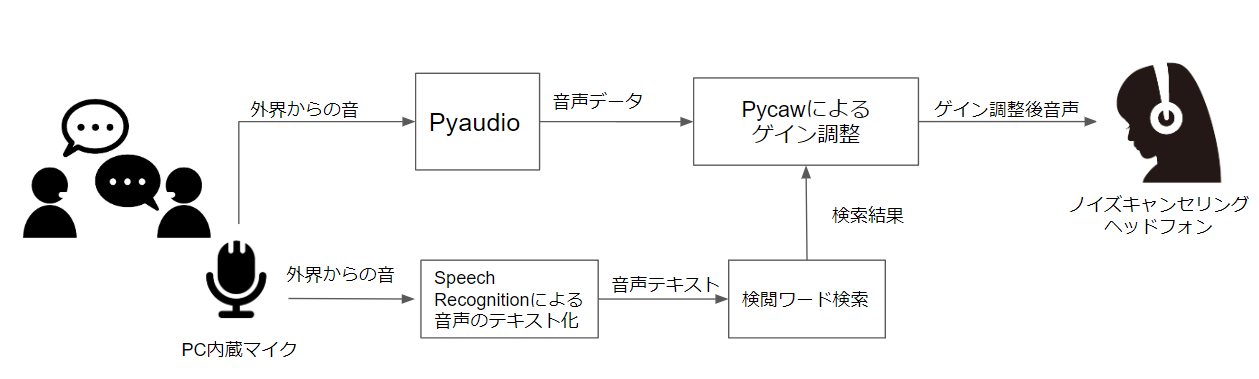
\includegraphics[width=90mm]{system.PNG}
    \caption{The device and the configuration}
    \label{fig:system}
    \end{center}
    \end{figure}

本研究で提案する装置の構成をFig.\ref{fig:system}に示す.
本装置はワイヤレスヘッドフォン(ag製 WHP01K),PC(DELL製 ALIENWARE 13(R3)),マイク(ALIENWARE 13(R3)内蔵マイク)によって構成される.
PCには,Pythonにより記述されたシステムが搭載されており,これによってマイクから入力される音に対して自動でゲイン調整を行う.
ワイヤレスヘッドフォンはノイズキャンセリング機能を有し,装置使用時はノイズキャンセリング機能を常にONの状態としている.
すなわちユーザーは外界からの音をマイクへの入力によってのみ得ることとなる.マイクへの入力として,基本的に人間による発話を想定している.
装置のマイクに入力された音声が,ゲイン調整されてユーザーに届くまでのシステム内の流れについて以下に述べる.

まず,マイクに入力された音声は,Google社のSpeech recognitionによってテキスト化される(Fig.\ref{fig:system}の下部).
次に,生成されたテキストは検閲ワード検索クラスに送られ,あらかじめ設定された検閲ワードがテキスト中に含まれていないかどうか検索が行われる.
もしテキスト中に検閲ワードが含まれていた場合は,含まれていた検閲ワードと,検閲ワードを見つけたという情報がゲイン調整クラスに送られる.
一方で,マイクに入力された音声はPythonライブラリ"Pyaudio"によってチャンクごとの音声データに分けられ,ゲイン調整クラスに送られる(Fig.\ref{fig:system}の上部).
ゲイン調整クラスでは,同じくPythonライブラリ"Pycaw"によって音声のゲイン調整が行われる.
このゲイン調整の度合いは発見した検閲ワードの種類に応じてあらかじめ設定することができる(例えば,”こんにちは”というワードを検閲ワードとし,ゲインを0とするトリガーとすることが事前に設定できる).
最後にゲイン調整済の音声がワイヤレスヘッドフォンに送られ,ユーザーは音声を聞くことができる.
\section{自動ゲイン調整装置の効果の検証}
\subsection{ゲイン調整効果の確認}
\subsubsection{実験概要}
装置によるゲインの自動調整の効果を確認するために,装置を装着した実験参加者に対して特定のキーワードを実験者から話しかけた際に,実験参加者に伝わる音声がどのように変化するかを確認する.
実験は対面で行い,実験者と実験参加者が机を挟んで対面で着席する状況で行われる(Fig.\ref{fig:env}).
後述する実験参加者のタスク遂行に与える影響の実験と同じように,「はじめてください」というキーワードで実験参加者に伝わる音声のゲイン0%(無音状態)にし,
「終わってください」というキーワードでゲインを100%(制限なし状態)とするように設定する.
実験者は装置を装着した実験参加者に対して,「始めてください」と言ったのち,実験参加者に対して30秒ごとに設定キーワードの含まれない言葉で声かけを行い,開始から3分後「終わってください」と声をかける.
\subsubsection{実験結果}
装置を装着した実験参加者に対して実験者から「始めてください」と発話した後,「終わってください」と発話するまでに装置を通してユーザーに届いた音声波形をFig.\ref{fig:voice}に示す
横軸が時間,縦軸が音声の振幅を示している.
また,同じ時間帯にFig.\ref{fig:env}のカメラで録音した,実験環境内の音声波形をFig.\ref{fig:outsidesound}に示す.
Fig.\ref{fig:voice}とFig.\ref{fig:outsidesound}を見ると実験者からの「始めてください」の声を検出してから「終わってください」の声を検出する間に発せられたアドバイスや環境音は完全にカットされていることがわかる.

\begin{figure}[htbp]
  \begin{center}
  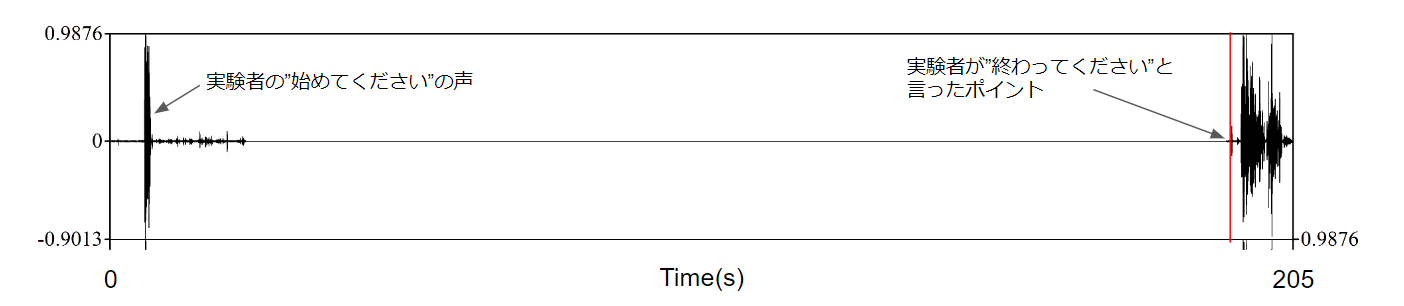
\includegraphics[width=90mm]{voice2.PNG}
  \caption{Audio waveform during automatic gain adjustment}
  \label{fig:voice}
  \end{center}
  \end{figure}

  \begin{figure}[htbp]
    \begin{center}
    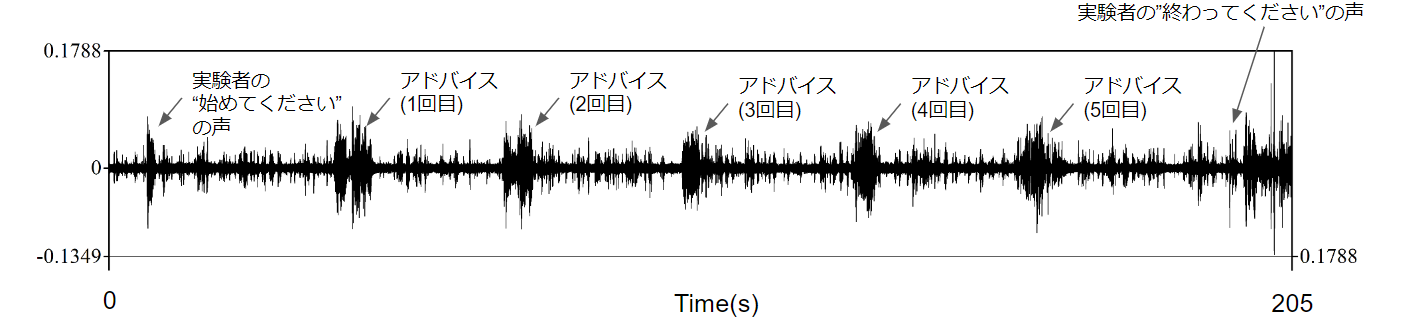
\includegraphics[width=90mm]{outersound.PNG}
    \caption{Audio waveform during automatic gain adjustment(outside sound)}
    \label{fig:outsidesound}
    \end{center}
    \end{figure}
\subsection{ユーザーのタスク遂行に与える影響}
\subsubsection{実験概要}
提案装置による音声の自動ゲイン調整がユーザーのタスク遂行に与える影響を調べるため,Alternative Uses Test\cite{AUT}を行った.
Alternative Uses Test(以下AUT)とは,実験参加者に日用品の新たな使い方のアイデアを思いつく限り列挙させるタスクである.
例えば日用品として「鉛筆」を提示する場合,通常であれば「メモを取る」等の用途が考えられる.
これに対してAUTでは通常の用途から逸脱する「黒板を示すのに使う」「箸の代わりとして使う」などの代替用途を実験参加者に発案させる(創造性の評価指標を乗せる).
回答されたアイデア群に対して,次の3つの指標を用いて評価する.
\begin{enumerate}
    \item[1)]流暢性:重複のないアイデア総数
    \item[2)]柔軟性:重複の無いアイデアの種類数
    \item[3)]独創性:アイデアの希少度合い.全実験参加者の全回答アイデア軍において,5%以下の出現率のアイデアを1点,1%以下の出現率のアイデアを2点とした
\end{enumerate}

AUT実施後,AUT結果から各実験参加者の実験結果による創造性指標(流暢性・柔軟性・独創性)を算出した.
その際に実験者の手作業によって,表現の異なる同義表現の正規化をおこなった.
流暢性は重複を除いた正規化済みの数とした.
正規化済みのアイデアを実験者の手作業により「衣類」,「工具」などの12個のカテゴリに分類し,重複しないカテゴリ総数を柔軟性スコアとした.
独創性は,正規化済みアイデアについて,出現率が全体アイデアの5%以下のものには1点を与え,点数の総和をスコアとした.
独創性スコアは,流暢性(アイデアの総数)と強い関係があることから,その関係をキャンセルしたスコアとして独創性を流暢性で割ったスコアを算出し,指標に加えた\cite{AUT2}.
提案装置は,作業者に対して話しかける人の音声をカットすることによって作業者の集中力を高めることを狙いとしている.
そこで本実験では,AUTの最中に実験者が実験参加者に口頭で代替用途を発案させるためのアドバイスを行うこととする.
本稿では18歳以上40歳未満の4人の男女(男性:3名,女性1名)に対して本検証実験を行った際の結果について報告する.

\subsubsection{実験環境}
実験は対面で行い,実験者と実験参加者が机を挟んで対面で着席する状況で行われる(Fig.\ref{fig:env}).
実験中における各人の身体運動(頭部および胸部運動)は実験参加者から見て左斜め前方に設置されたビデオカメラ(DJI製 Osmo Pocket)により記録する.
記録したデータは各人の活動量の分析のために使用する.

\begin{figure}[htbp]
    \begin{center}
    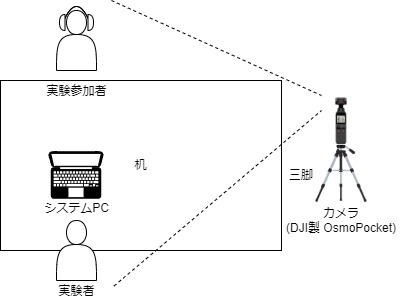
\includegraphics[width=80mm]{configuration.jpg}
    \caption{Experiment environment}
    \label{fig:env}
    \end{center}
    \end{figure}
\subsubsection{実験の流れ}
実験の流れを以下に示す
\begin{enumerate}
    \item 実験参加者が提案装置を装着する
    \item 実験者が実験参加者にAUTの実施方法を説明する
    \item 実験者が実験参加者にお題となる日用品の名称を伝える.実験者からの「はじめてください」の言葉とともに,実験参加者はAUTを開始する
    \item 随時,実験者から実験参加者へ,代替用途を発案するためのアドバイスを口頭で伝える
    \item AUT開始から3分経過した時点で,実験者の「終了してください」の言葉とともにAUTを終了する
    \item (2)から(4)をもう一度繰り返す
\end{enumerate}

実験参加者は,AUTのお題として,1回目の試行では「ボールペン」,2回目の試行では「靴下」について代替用途を回答するよう指示する.
実験参加者は発案した代替用途をA4サイズのフォームに逐次記入する.
また,AUT実施中の実験者からのアドバイスは,お題に依存するもの(お題が靴下であれば「素材が布であることを考えると面白いアイデアが思いつくかもしれません.」等)と,
お題に依存しないもの(「誰が使うかを考えてみるといいアイデアが思いつくかもしれません」等)を組み合わせ,AUT開始から30秒毎に1回ずつ計5回口頭で行う.
AUT終了後,実験参加者は心理アンケートに回答する.
アンケート結果は実験参加者のアイデア出しへの自己評価や,実験者に対する印象などを調査するために使用する.

\subsubsection{実験条件}
実験を行うにあたりシステム強使用条件とシステム弱使用条件の2条件を設ける.
システム強使用条件では,「はじめてください」というキーワードをゲインを0%(無音状態)にするトリガーとし,
「終わってください」というキーワードをゲイン100%(制限なし状態)とするトリガーとする.
すなわち,この条件では,具体的な実験に対する説明を除き,AUT実施中にマイクに入力された音声が全てカットされる.
また,システム弱使用条件では,ゲイン調整を行うトリガーを設けず,実験の全ての段階でマイクに入力された音声はそのまま実験参加者に伝達される.
今回の実験においては,各条件に付き2名ずつ実験を実施した.実験参加者にはどちらの条件が適用されたかについて知らされなかった.

\subsubsection{実験結果}
システム強使用条件とシステム弱使用条件におけるAUT課題の創造性指標の結果をそれぞれTable.\ref{table:week}, Table.\ref{table:strong}に示す.
\begin{table}[htbp]
    \caption{システム弱使用条件でのAUT課題における創造性指標}
    \label{table:week}
    \centering
    \begin{tabular}{lccc}
      \hline
      \multicolumn{4}{c}{試行1回目 お題:ボールペン} \\
      \hline
      創造性指標  & 実験参加者1  &  実験参加者2  &  平均 \\
      \hline
      流暢性  & 4  & 7 & 5.5 \\
      柔軟性  & 3   & 6  & 4.5 \\
      独創性  & 1  & 4 & 2.5 \\
      独創性/流暢性  & 0.25 & 0.57 & 0.41 \\
      \hline
      \multicolumn{4}{c}{試行2回目 お題:靴下} \\
      \hline
      創造性指標  & 実験参加者1  &  実験参加者2  &  平均 \\
      \hline
      流暢性  & 6  & 6 & 6 \\
      柔軟性  & 5   & 4  & 4.5 \\
      独創性  & 2  & 3 & 2.5 \\
      独創性/流暢性  & 0.33 & 0.5 & 0.42 \\
      \hline
    \end{tabular}
  \end{table}

\begin{table}[h]
    \caption{システム強使用条件でのAUT課題における創造性指標}
    \label{table:strong}
    \centering
    \begin{tabular}{lccc}
      \hline
      \multicolumn{4}{c}{試行1回目 お題:ボールペン} \\
      \hline
      創造性指標  & 実験参加者3  &  実験参加者4  &  平均 \\
      \hline
      流暢性  & 8  & 9 & 8.5 \\
      柔軟性  & 4   & 4  & 4 \\
      独創性  & 3  & 4 & 3.5 \\
      独創性/流暢性  & 0.38 & 0.44 & 0.41 \\
      \hline
      \multicolumn{4}{c}{試行2回目 お題:靴下} \\
      \hline
      創造性指標  & 実験参加者3  &  実験参加者4  &  平均 \\
      \hline
      流暢性  & 7  & 9 & 8 \\
      柔軟性  & 5   & 5  & 5 \\
      独創性  & 6  & 6 & 6 \\
      独創性/流暢性  & 0.86 & 0.67 & 0.76 \\
      \hline
    \end{tabular}
\end{table}

\section{ディスカッション}
1回目の試行,2回目の試行の両方で,システム強使用条件のほうがAUTにおける流暢性(アイデアの総数)が高くなる傾向が見えた.
この傾向が現れた原因としてAUT中に実験者からのアドバイスをカットしたことにより,実験参加者が気を散らさず集中してアイデア出しに取り組むことができ,結果として思いついたアイデアの数が多くなった可能性が考えられる.
今回はアドバイスを一律にカットしたが,カットするアドバイスを選択したり,アイデアが出尽くしたことを検知して,アドバイスのカットを中止したりする機能が追加できれば,更に流暢性を向上させることができるかもしれない.
柔軟性に関しては,システム強使用条件と弱使用条件の間でほとんど変化が見れらなかった.
独創性については2回目の施行のみ,システム強使用条件の方が独創性/流暢性の値が高くなる傾向が見えた.
これはAUT中に実験者からのアドバイスをカットしたことにより,実験参加者は実験者が提示したアドバイスに思考が引っ張られず,結果としてアイデアの独自性が高くなった可能性が考えられる.
今回はシステム強使用条件とシステム弱使用条件で,それぞれ別の参加者がAUTを行ったが独創性や流暢性の値は個人による差異があると考えられ,そのような差異を包括するような実験系を考えていく必要がある.
また,今回は実験前にAUTのプレテストを行うことはしなかったが,創造性指標を正確に捉えるため,今後導入することを考えていく.

\section{結言}
本稿では特定のキーワードに対応して音声のゲインを自動調整する装置を開発した.
また,この装置を装着した実験参加者にシステム強使用条件とシステム弱使用条件の2条件下でAlternative Uses Testを行ってもらうことで,提案装置がユーザのタスク遂行に与える影響を検討した.
本稿で示した結果は,各条件の参加者2名ずつの事例報告であるが,システム強使用条件においてAUTの創造性指標の一つである流暢性が高くなる傾向が見えた.
発表では,より多数の実験参加者における傾向について統計的な議論を行う予定である.
また,心理アンケートの結果やAUT実施時の実験参加者の身体動作についても分析を行い,提案装置の有効性について包括的に議論する予定である.
%
%
%参考文献
\begin{thebibliography}{99}
\bibitem{noise}西村 正治, アクティブノイズコントロールの現状, 計測と制御, 2012, 51 巻, 12 号, p. 1105-1109
\bibitem{impact}細井 裕司, 補聴器この20年間の進歩, 日本耳鼻咽喉科学会会報, 2011, 114 巻, 12 号, p. 905-911
\bibitem{AUT}Guilford, J. P., “The nature of human intelligence”, New York, NY: McGraw-Hill,
1967
\bibitem{AUT2}中原和洋,「アイデア創出の促進および阻害要因の解消」,
ユニシス技報,日本ユニシス,第139号,2019年53月
\end{thebibliography}
%
%
%
\end{document}

